\documentclass[dvisvgm,tikz,margin=2pt]{standalone}
\usepackage{amsmath,amssymb,amsthm,mathtools}
\usepackage{tikz}
\usetikzlibrary{positioning,calc}
\usepackage{xcolor}
\newcommand{\R}{\mathbb{R}}
\newcommand{\Q}{\mathbb{Q}}
\newcommand{\abs}[1]{\lvert #1\rvert}
\newcommand{\norm}[1]{\lVert #1\rVert}
\newcommand{\RSSP}{\textsc{Riesz-Subset}}
\newcommand{\MIS}{\textsc{Independent-Set}}
\newcommand{\sgnspin}{\{-1,+1\}}
\begin{document}
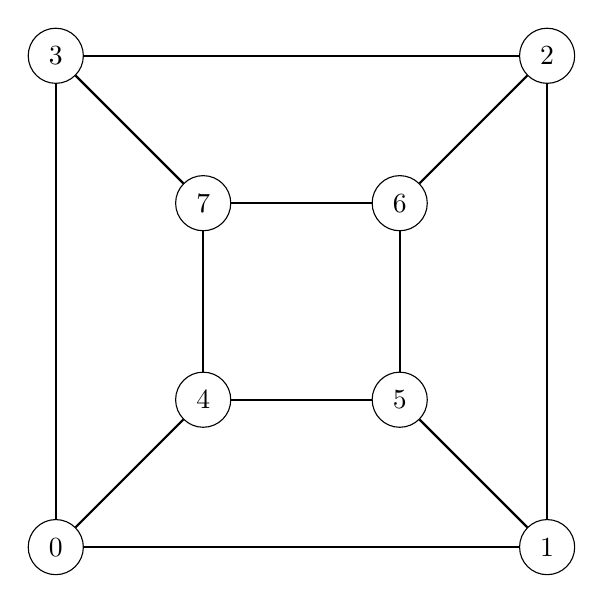
\begin{tikzpicture}[scale=0.78,
  vtx/.style={circle,draw,minimum size=7mm,inner sep=0pt,fill=white},
  ed/.style={thick}]
  \node[vtx] (v0) at (-4,-4) {0};
  \node[vtx] (v1) at ( 4,-4) {1};
  \node[vtx] (v2) at ( 4, 4) {2};
  \node[vtx] (v3) at (-4, 4) {3};
  \node[vtx] (v4) at (-1.6,-1.6) {4};
  \node[vtx] (v5) at ( 1.6,-1.6) {5};
  \node[vtx] (v6) at ( 1.6, 1.6) {6};
  \node[vtx] (v7) at (-1.6, 1.6) {7};
  \draw[ed] (v0)--(v1)--(v2)--(v3)--(v0);
  \draw[ed] (v4)--(v5)--(v6)--(v7)--(v4);
  \draw[ed] (v0)--(v4);
  \draw[ed] (v1)--(v5);
  \draw[ed] (v2)--(v6);
  \draw[ed] (v3)--(v7);
\end{tikzpicture}
\end{document}
